%%%% ijcai09.tex

\typeout{IJCAI-09 Instructions for Authors}

% These are the instructions for authors for IJCAI-09.
% They are the same as the ones for IJCAI-07 with superficical wording
%   changes only.

\documentclass{article}
% The file ijcai09.sty is the style file for IJCAI-09 (same as ijcai07.sty).
\usepackage{ijcai09}

% Use the postscript times font!
\usepackage{times}

\usepackage{graphicx}
\usepackage{float}
\usepackage{dblfloatfix}

% the following package is optional:
%\usepackage{latexsym} 

% Following comment is from ijcai97-submit.tex:
% The preparation of these files was supported by Schlumberger Palo Alto
% Research, AT\&T Bell Laboratories, and Morgan Kaufmann Publishers.
% Shirley Jowell, of Morgan Kaufmann Publishers, and Peter F.
% Patel-Schneider, of AT\&T Bell Laboratories collaborated on their
% preparation.

% These instructions can be modified and used in other conferences as long
% as credit to the authors and supporting agencies is retained, this notice
% is not changed, and further modification or reuse is not restricted.
% Neither Shirley Jowell nor Peter F. Patel-Schneider can be listed as
% contacts for providing assistance without their prior permission.

% To use for other conferences, change references to files and the
% conference appropriate and use other authors, contacts, publishers, and
% organizations.
% Also change the deadline and address for returning papers and the length and
% page charge instructions.
% Put where the files are available in the appropriate places.

\title{UAV Character Classification Using a Convolutional Neural Net}
\author{Tyler Miller, Cory Sivek, Jarett Iverson \\
CS 478 Fall 2018 \\
Department of Computer Science\\
Brigham Young University}

\begin{document}

\maketitle

\begin{abstract}
  Character recognition is one of the classical problems often used as a benchmark for various machine learning algorithms. In this project we investigate the feasibility of character recognition by an in-flight unmanned aerial vehicle (UAV) using a convolutional neural net (CNN). Recognition from a UAV presents two unique challenges: 1: the character is in an unknown orientation, and 2: clarity of the image is affected by the motion of the craft. In this report we compare various approaches to this problem, and the learning model we found to be most effective. Through our experiments, we were able to achieve 98\% validation accuracy and 88\% test accuracy. 
\end{abstract}

\section{Introduction}

The AUVSI competition is an international system engineering competition. It tests how well 
teams can interface a variety of sensors, software and actuators. The three main challenges 
presented by the AUVSI competition are: autonomous flight, dynamic obstacle avoidance, and 
object detection classification and localization. To object detection, teams must image the 
ground from the flying UAV and autonomously identify relevant targets. ‘Targets’ are composed 
of colored shapes with an uppercase letter in the middle. Figure \ref{fig:sampleTarget} shows an example of a 
competition target.

\begin{figure}[H]
  \begin{center}
  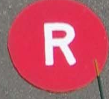
\includegraphics[width=0.4\linewidth]{./figs/target-R.png}
  \caption{Sample object target from AUVSI 2017 competition}
  \label{fig:sampleTarget}
  \end{center}
\end{figure}

The largest challenge of target classification is reliably identifying the letters on these targets. 
Target letters are unknown at flight time, but must be classified while the UAV is still in the air.
With the craft flying anywhere between 100-200 feet of altitude, targets are relatively small on the
raw image. Thus letters are pixelated and have a high degree of motion blur since the imaging system 
is unable to focus on such a small object. Besides this high degree of motion blur, letters may also 
be at any rotation. The orientation of the target is unknown and could be imaged by the craft while 
it pursues any number of headings, meaning it’s impossible for reliably assume a specific letter 
orientation.

These challenges in mind, the AUVSI team has already made a number of strides in addressing them. Below 
(Figure \ref{fig:imagingFlowchart}) is an example flowchart of the autonomous object detection system under development by AUVSI. With 
posterization, canny edge and blob detection, images can be reliably cropped down to just individual 
targets. From here they can be fed into our CNN letter classifier (shown in green), before being sent 
to the judges. 

\begin{figure}[H]
  \begin{center}
  
\includegraphics[width=\linewidth]{./figs/auvsiImagingFlowchart.png}
  \caption{Autonomous object classification block diagram (the problem portion tackled in this paper is in green)}
  \label{fig:imagingFlowchart}
  \end{center}
\end{figure}

\section{Methods}

In this section we discuss the various methods used for the classification problem.

\subsection{Dataset}

Ideally our dataset would purely comprise of target images taken by the UAV, and cropped by BYU 
AUVSI’s autonomous system. Unfortunately, the image volume required for adequate model training 
simply wasn’t available. To maximize our productivity, we generated two synthetic datasets. One 
‘basic’ dataset of about 2,000 images and one ‘complex’ dataset of around 15,000 images. With 
the basic dataset we were able to train many different models quickly. This allowed us to take a 
broad approach to the best strategy before narrowing down to a single model and fine tuning it with 
the complex dataset.

Both of these datasets made some key assumptions. First, as per AUVSI rules, the letters would only 
be in upper case. Second, we assumed the autonomous cropping algorithm would work reliably and place 
the target letter near center frame of the image. Third, as discussed in the introduction, the letter 
could be in any orientation with varying degrees of motion blur.

With these assumptions in mind, we generated the basic dataset using Adobe Photoshop’s javascript API. 
A sample image from the basic dataset is shown  in Figure \ref{fig:basicDataset}. As shown, the basic dataset was simple 
black and white. We created an image for each letter at various rotation steps and blur levels. While 
this dataset greatly simplifies the overall problem, it contains some of the key challenges that make 
this problem space unique.

\begin{figure}[H]
  \begin{center}
  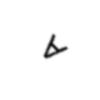
\includegraphics[width=0.7\linewidth]{./figs/basicDatasetSample.jpeg}
  \caption{A training image for the letter 'A' from the basic dataset}
  \label{fig:basicDataset}
  \end{center}
\end{figure}

The complex dataset on the other had, was more true-to-life. While Photoshop’s scripting API had a lot 
of powerful features, we found it to be too slow when generating the larger dataset. For this reason, 
we moved over to Python’s imaging library (PIL) to generate the 15k image complex dataset. A sample image 
from this dataset is shown in Figure \ref{fig:complexDataset}. As displayed, this dataset continued to rotate and apply varying 
blur to the letter, as with the basic dataset. However, it also changed the color of the letter and placed 
a random target shape (square, rectangle, etc) of random color behind the letter. In this random generation, 
it was ensured that the color of the letter was not too similar to the color of the shape.

\begin{figure}[H]
  \begin{center}
  
\includegraphics[width=0.7\linewidth]{./figs/complexDatasetSample.jpeg}
  \caption{A training image for the letter 'A' from the complex dataset}
  \label{fig:complexDataset}
  \end{center}
\end{figure}

Using these two datasets, we were able to successfully test a multitude of configuration options quickly 
using the basic dataset, and fine tune our best model with the more realistic complex dataset.

\subsection{Model Selection}

It was immediately apparent that the optimal solution involved a Convolutional Neural Network (CNN) 
considering that we were dealing with image data, but it was not clear what model would fit best. After 
looking at different libraries and tools for CNNs, and after consulting Dr. Bryan Morse, we had decided 
to learn and use PyTorch as the underbelly of our solution. 

Our strategy going forward was to research into existing CNN models that others have made for PyTorch 
and also jury-rig pre-trained models to solve our specific problem. We found a variety of these pre-trained 
models and ran them on our dataset using default parameters and compared the first couple of epochs (see 
Figures \ref{fig:modelValAcc} and \ref{fig:modelTrainTime}).

\begin{figure*}
  \begin{center}
  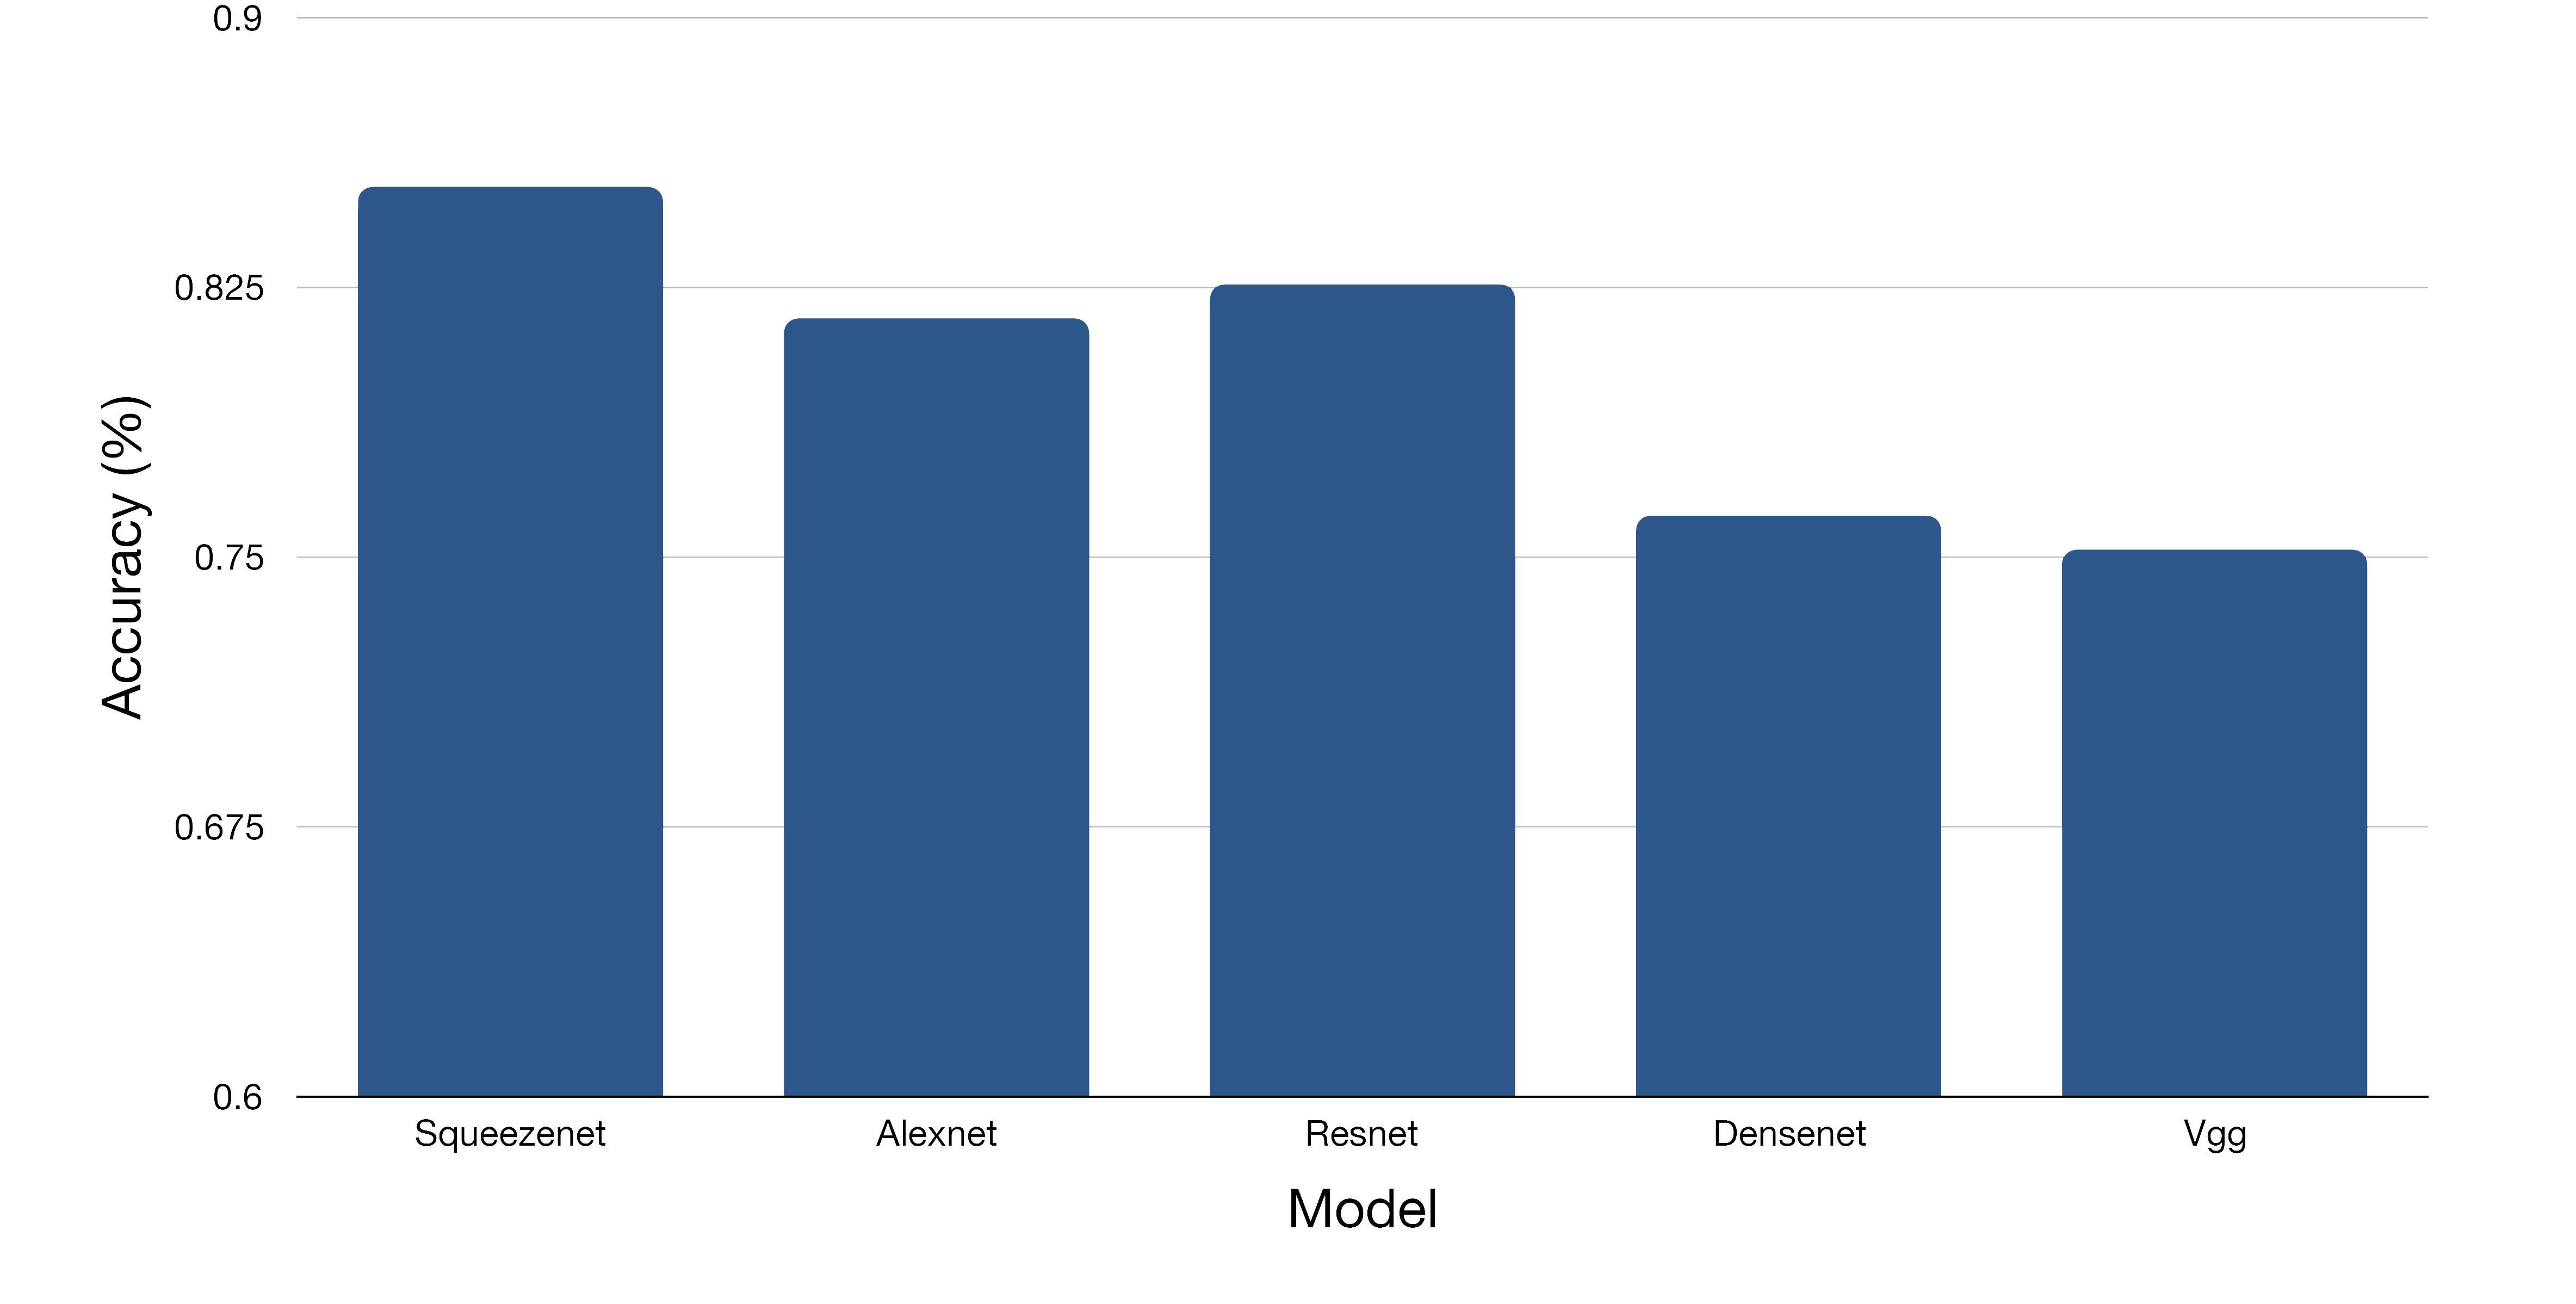
\includegraphics[width=\textwidth]{./figs/pretrainedAccuracyCropped.png}
  \caption{Model validation accuracy after 15 epochs}
  \label{fig:modelValAcc}
  \end{center}
\end{figure*}

\begin{figure*}
  \begin{center}
  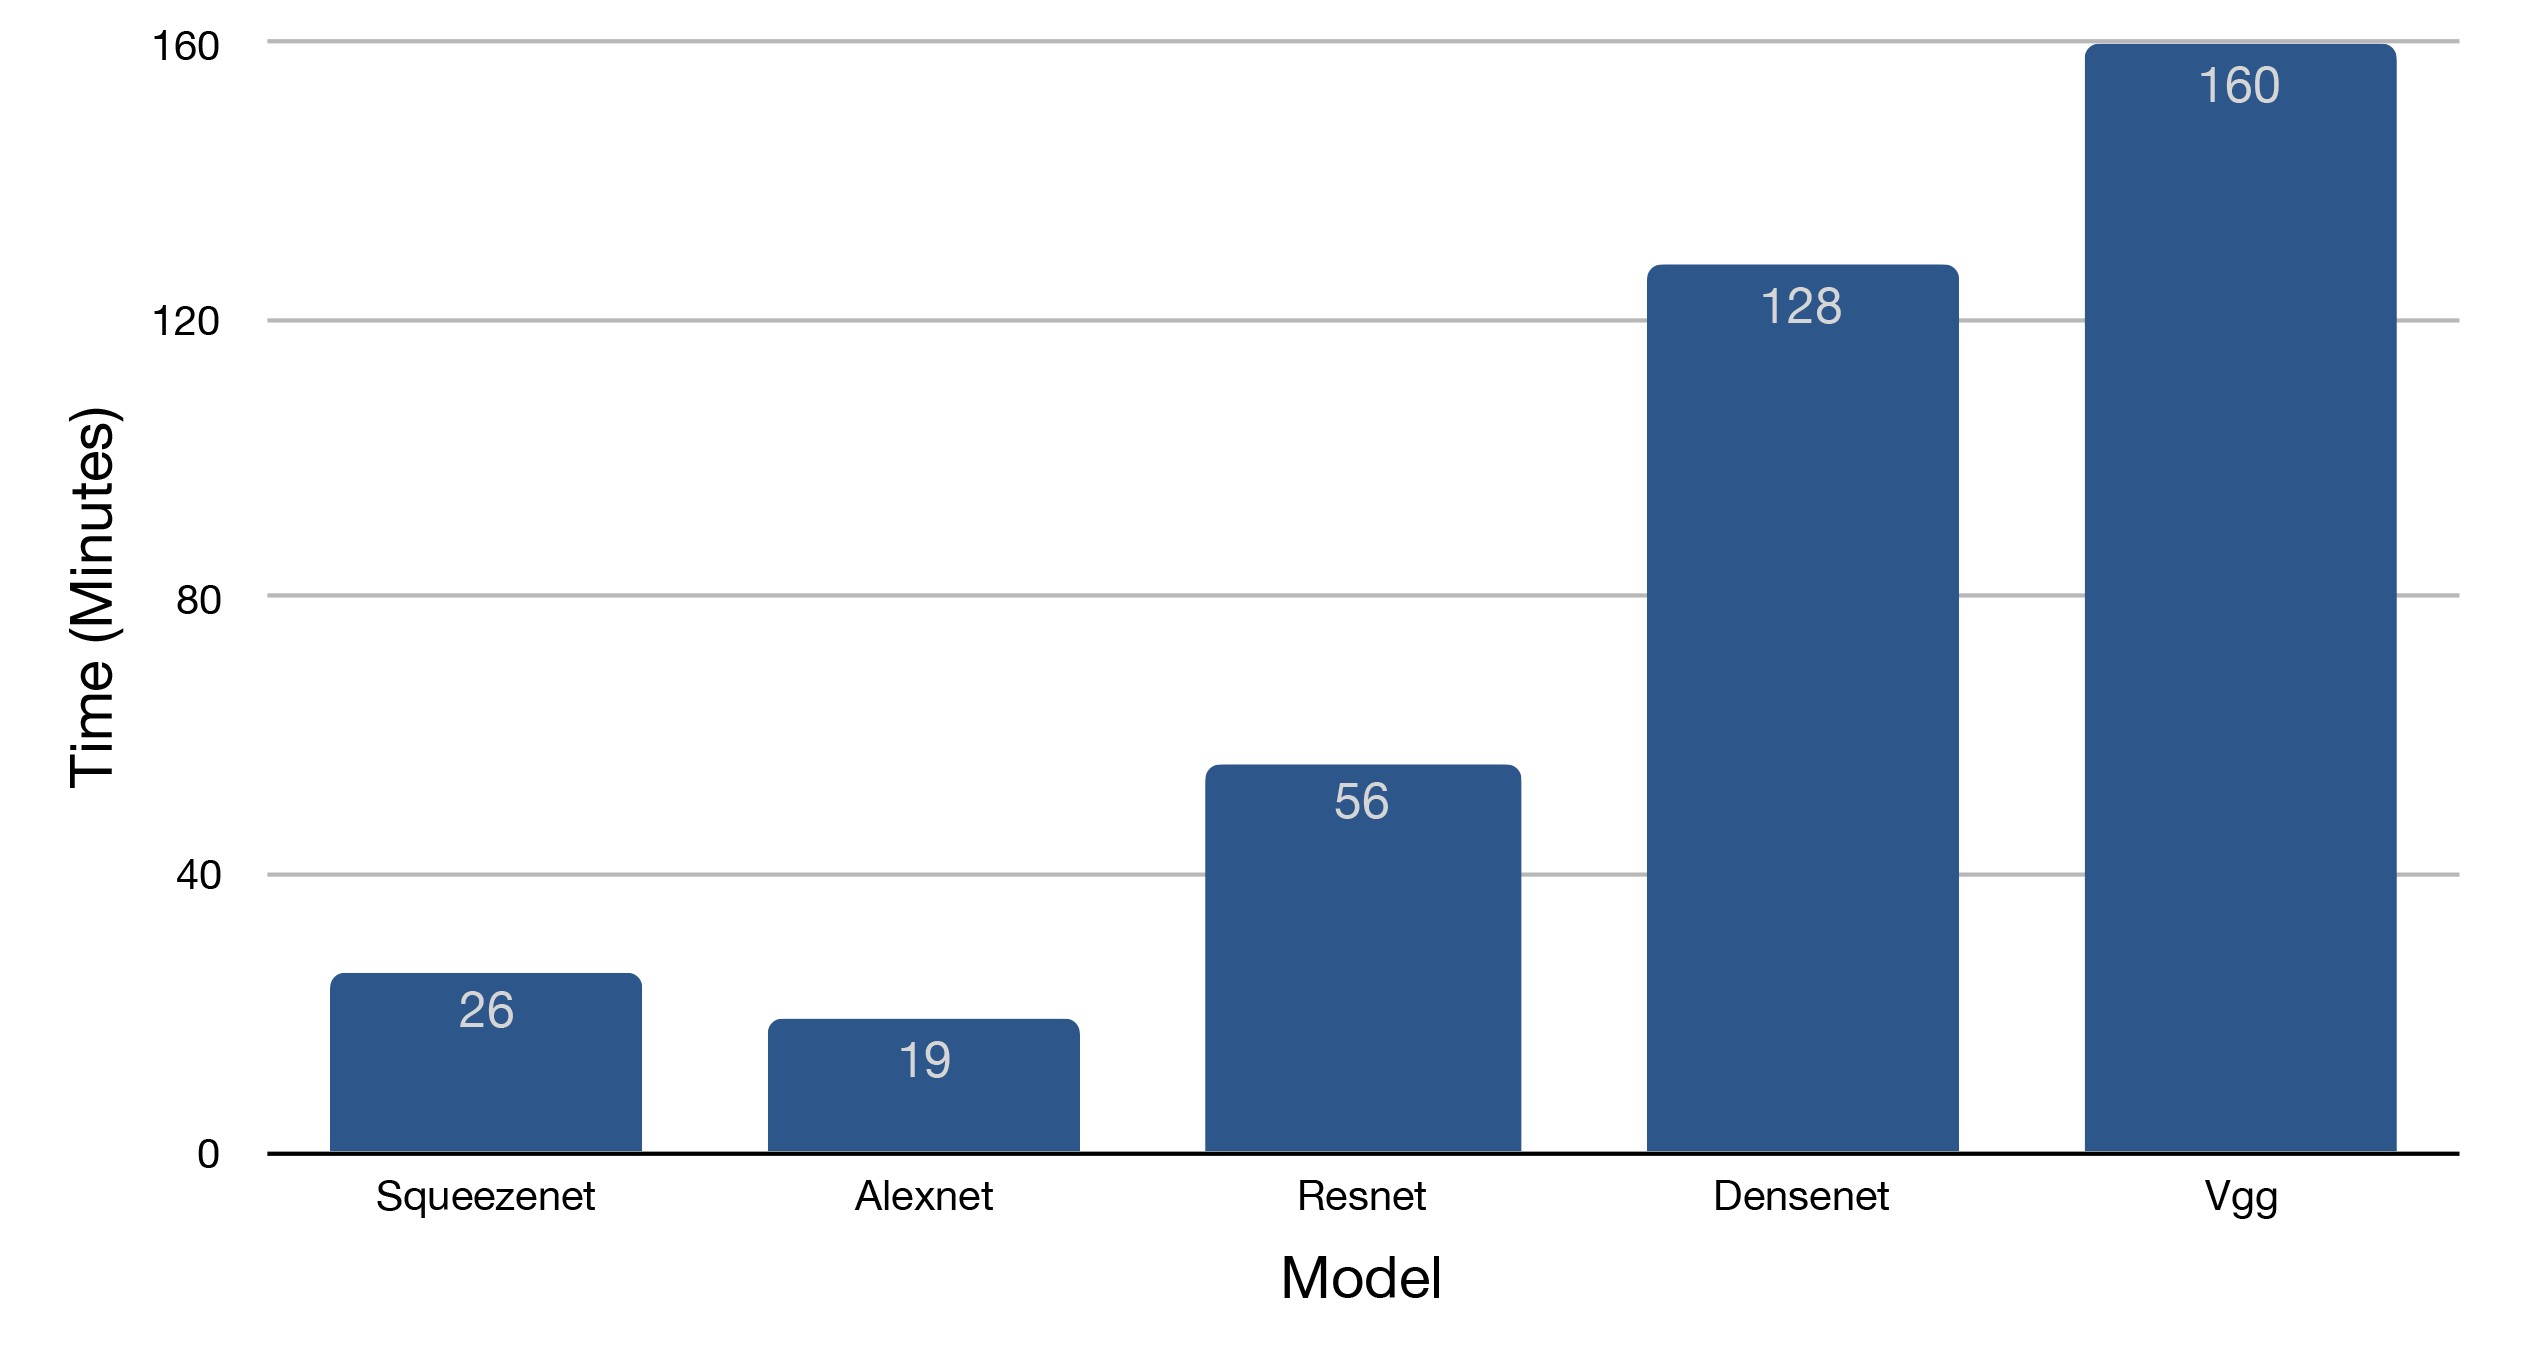
\includegraphics[width=\textwidth]{./figs/pretrainedTimeCropped.png}
  \caption{Model train time for 15 epochs}
  \label{fig:modelTrainTime}
  \end{center}
\end{figure*}

\begin{figure*}[b]
  \begin{center}
  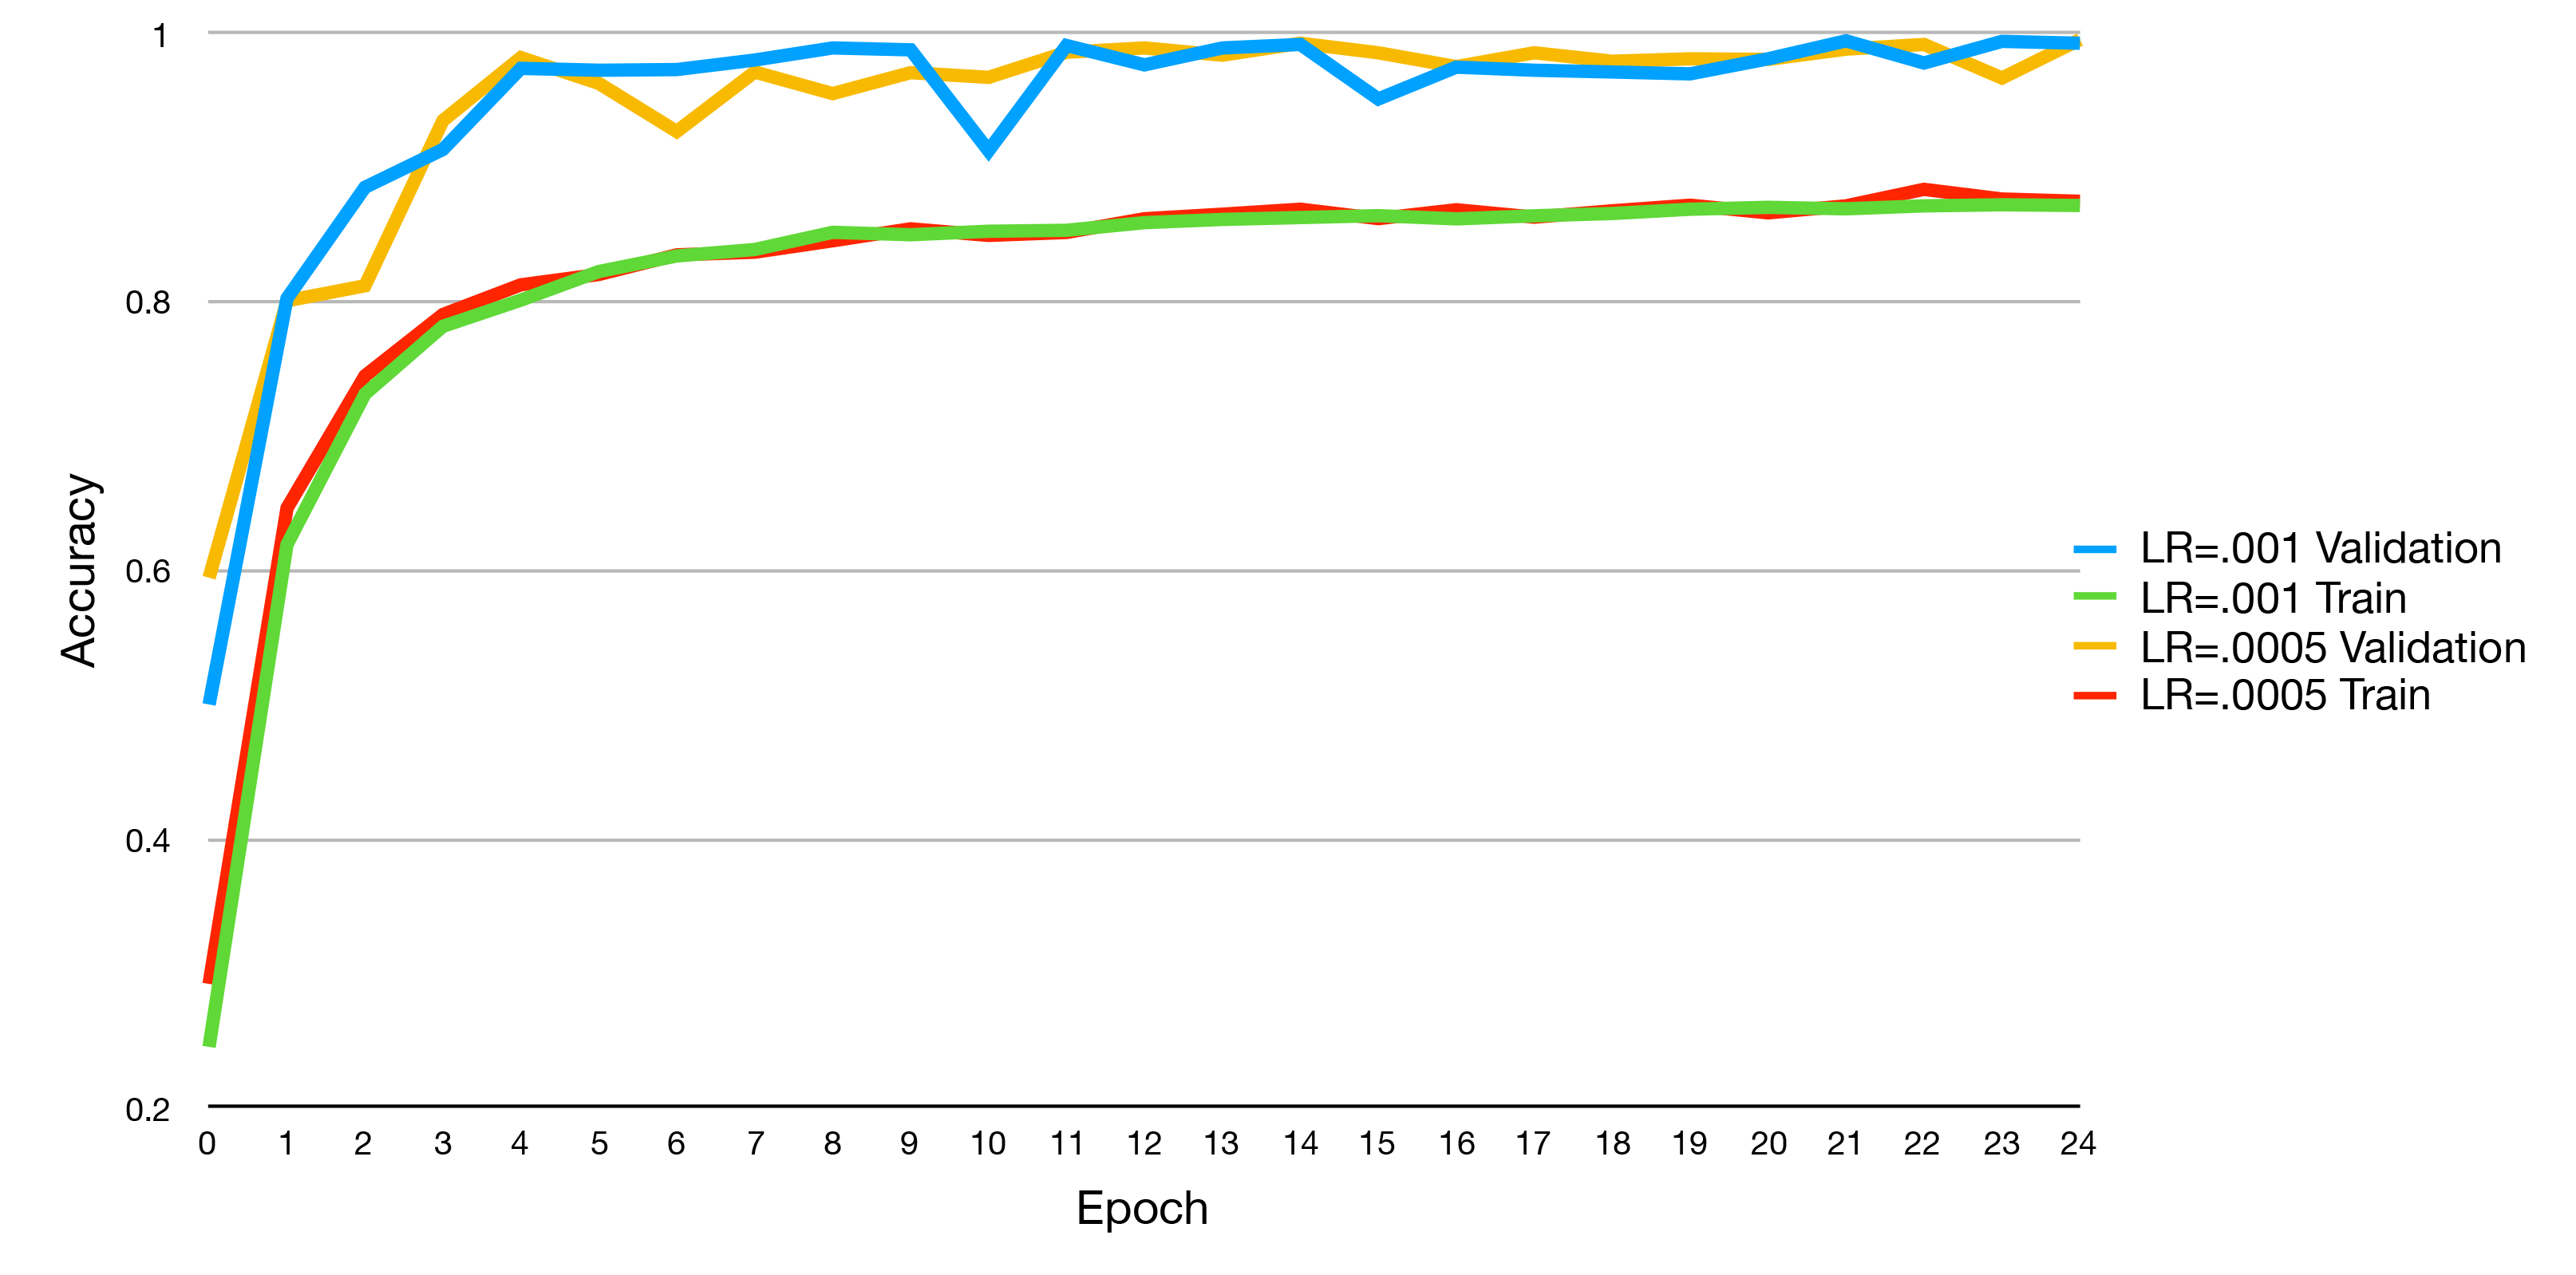
\includegraphics[width=\textwidth]{./figs/extendedSqueeze-learningRatesCropped.png}
  \caption{Extended squeeze Train and Validation accuracies over 25 Epochs with two learning rates}
  \label{fig:extSqueezeAcc}
  \end{center}
\end{figure*}

It is considerable to note that none of us had working GPUs on our computers and had done the tests 
running on CPUs alone. This factored into our decision to choose Squeezenet as a good base Model to 
further develop with, as it proved to be one of the fastest models to train with one of the best 
accuracies. We considered that Squeezenet works very well on our particular dataset because each squeeze 
(image compression) does not lose very much information as our images consist of simple flat objects 
with 2 to 3 colors.

\subsection{Model Tuning}

After selecting Squeezenet as a base to derive our own model from, we started to modify the squeezenet 
model and learn it on our dataset. At one point while tuning our model, we managed to get PyTorch working 
in the animation labs with a working GPU, so we ran our test for longer epochs. The following were the 
main modifications we made per train of the CNN model:

\subsubsection{Reduce the model to a single squeeze and expand cycle}

This cycle (referred to as a Fire module for squeezenet) will first run a few 1x1 convolutions to reduce 
the amount of features, and then it runs a few 1x1 and 3x3 convolutions to expand more features back into 
the model. This test obviously didn’t help with the learning, but we wanted to see what a single fire 
module does by itself.

\subsubsection{Removed duplicate Fire modules for each layer}

We recognized that there were multiple Fire modules being run before each MaxPool and each condensing 
of the total image size. Considering that we were working on simpler images with less features, we wanted 
to see if taking out anything would improve upon our accuracy. Our tests suggested that we always got 
worse accuracy the more we took out.

\subsubsection{Added an additional Fire module and squeeze layer}

So taking from what we learned in our previous test, we decided to add an additional layer of Fires 
and a MaxPool. We didn’t have significantly better results but we did reach our highest accuracy on our 
validation set with this configuration.

\subsubsection{Converting all input images to single channel images (black and white)}

We attempted to make the input simpler for our model by converting the Color in our dataset to black 
and white beforehand. We were surprised to find that reducing the input from 3 channels per pixel to 
1 channel reduced our accuracy by a significant amount. Apparently, the color separation is useful 
for the learned models.


\subsubsection{Changing the optimizer function}

PyTorch supports simply changing the optimizer function in any neural network model and comes with a 
variety in their libraries. So we tested our model on the defaults of optimizer functions: Adadelta, 
Adagrad, Adam, Adamax, SparseAdam, Average SGD, SGD, and L-BFGS. From our tests, Stochastic Gradient 
Descent (SGD) was the optimal optimizer function as most of the other functions never allowed the 
model to surpass 10\% accuracy.

\subsubsection{Modifying the Learning Rate}

Finally, we tested training our model with different learning rates on the SGD optimizer function. 
Our tests revealed that the learning rate had little effect on the accuracy of the model as we were 
already reaching validation accuracies of ~99\%.

\section{Final Results}

After determining that the model with an additional Squeeze and Fire layer gave us our highest accuracy 
with the basic dataset, we tested that model on the complex dataset with 15,000 images. This set was 
split 85/15 between validation and training. We also ran this model for an increased number of epochs, 
up to 25 from the 15 we used in testing the models on the basic set. The results are shown in Figure \ref{fig:extSqueezeAcc} 
This produced our highest validation accuracy of 98.17\%, and a test set accuracy of 73.23\%. For these runs 
we were able to utilize a machine capable of GPU processing the data so the runtime was 2 minutes 49 
seconds, a huge increase in speed compared to our previous tests. We observed no significant differences 
in changing the learning rate for this model.

\section{Conclusion and Future Work}

Through our experimentation we were able to build a model that can be used to classify characters 
with high accuracy even in spite of rotation and blurring. This model could work reasonably well 
for the AUVSI competition, but we know that further improvements can be made. One of the major 
difficulties we faced in our testing was the high runtime of training our models. We are in the 
processes of generating a larger set of 2.2 million images, and with the accelerated GPU performance 
we will be able to train on this set and potentially test an even higher number of epochs to optimize 
accuracy. We also need to include real datasets of cropped images taken by the UAV as there may be 
some discrepancy between them and those we artificially generated.  

\end{document}
